\documentclass{article}

\usepackage[utf8]{inputenc}
\usepackage[T1]{fontenc}
\usepackage[francais]{babel}
\usepackage{url}
\usepackage{color}
\usepackage{verbatim}
\usepackage{amsmath,amssymb,amsfonts}
\usepackage{graphicx}
\usepackage[french]{algorithm2e}
\usepackage{geometry}
\usepackage{enumitem}
\usepackage{listings}
\frenchbsetup{StandardLists=true}
\lstset{language=SQL}
\geometry{hmargin=2.5cm, vmargin=2.5cm}

\title{Introduction aux Réseaux TP2 : \\ Etude des protocoles ARP et ICMP}
\author{Line \bsc{POUVARET}, Mickaël \bsc{TURNEL}}
\date{2015-2016}


\begin{document}

\maketitle

\section*{2.1 Etude des protocoles de niveau 3}

\subsection*{2.1.1 Le protocole ARP}

\subsubsection*{\underline{Syntaxe des paquets ARP}}

\begin{itemize}\renewcommand{\labelitemi}{$\bullet$}

	\item Entête Ethernet : ff ff ff ff ff ff 00 10 18 89 e9 7a 08 06 (14 premiers octets) ET les 18 derniers octets ; les 7 premiers octets correspondent à l'adresse de la cible, et les 7 suivants à l'adresse de la source.
Données ARP : tous les octets entre les deux parties de l'entête Ethernet.
	\item Dans le champ type de l'entête Ethernet II on a ARP (0x0806).

	\item Les champs d'ARP :
	\begin{itemize}\renewcommand{\labelitemi}{$\bullet$}
		\item Hardware type correspond au type de matériel utilisé (ici Ethernet (1))
		\item Protocol type correspond au protocol utilisé (ici IP (0x800))
		\item Hardware size correspond à la taille du protocole matériel (6 octets pour MAC)
		\item Protocol size correspond à la taille du protocole (4 octets pour IPv4)
		\item Opcode correspond au type de message (requête ou réponse)
		\item Sender MAC address correspond à l'adresse Ethernet de l'envoyeur du paquet
		\item Sender IP address correspond à l'adresse Internet de l'envoyeur
		\item Target MAC address correspond à l'adresse Ethernet du destinataire (inconnu lors d'une requête)
		\item Target IP address correspond à l'adresse Internet du destinataire
	\end{itemize}
	\item Le paquet ARP se trouve dans le champ Data.

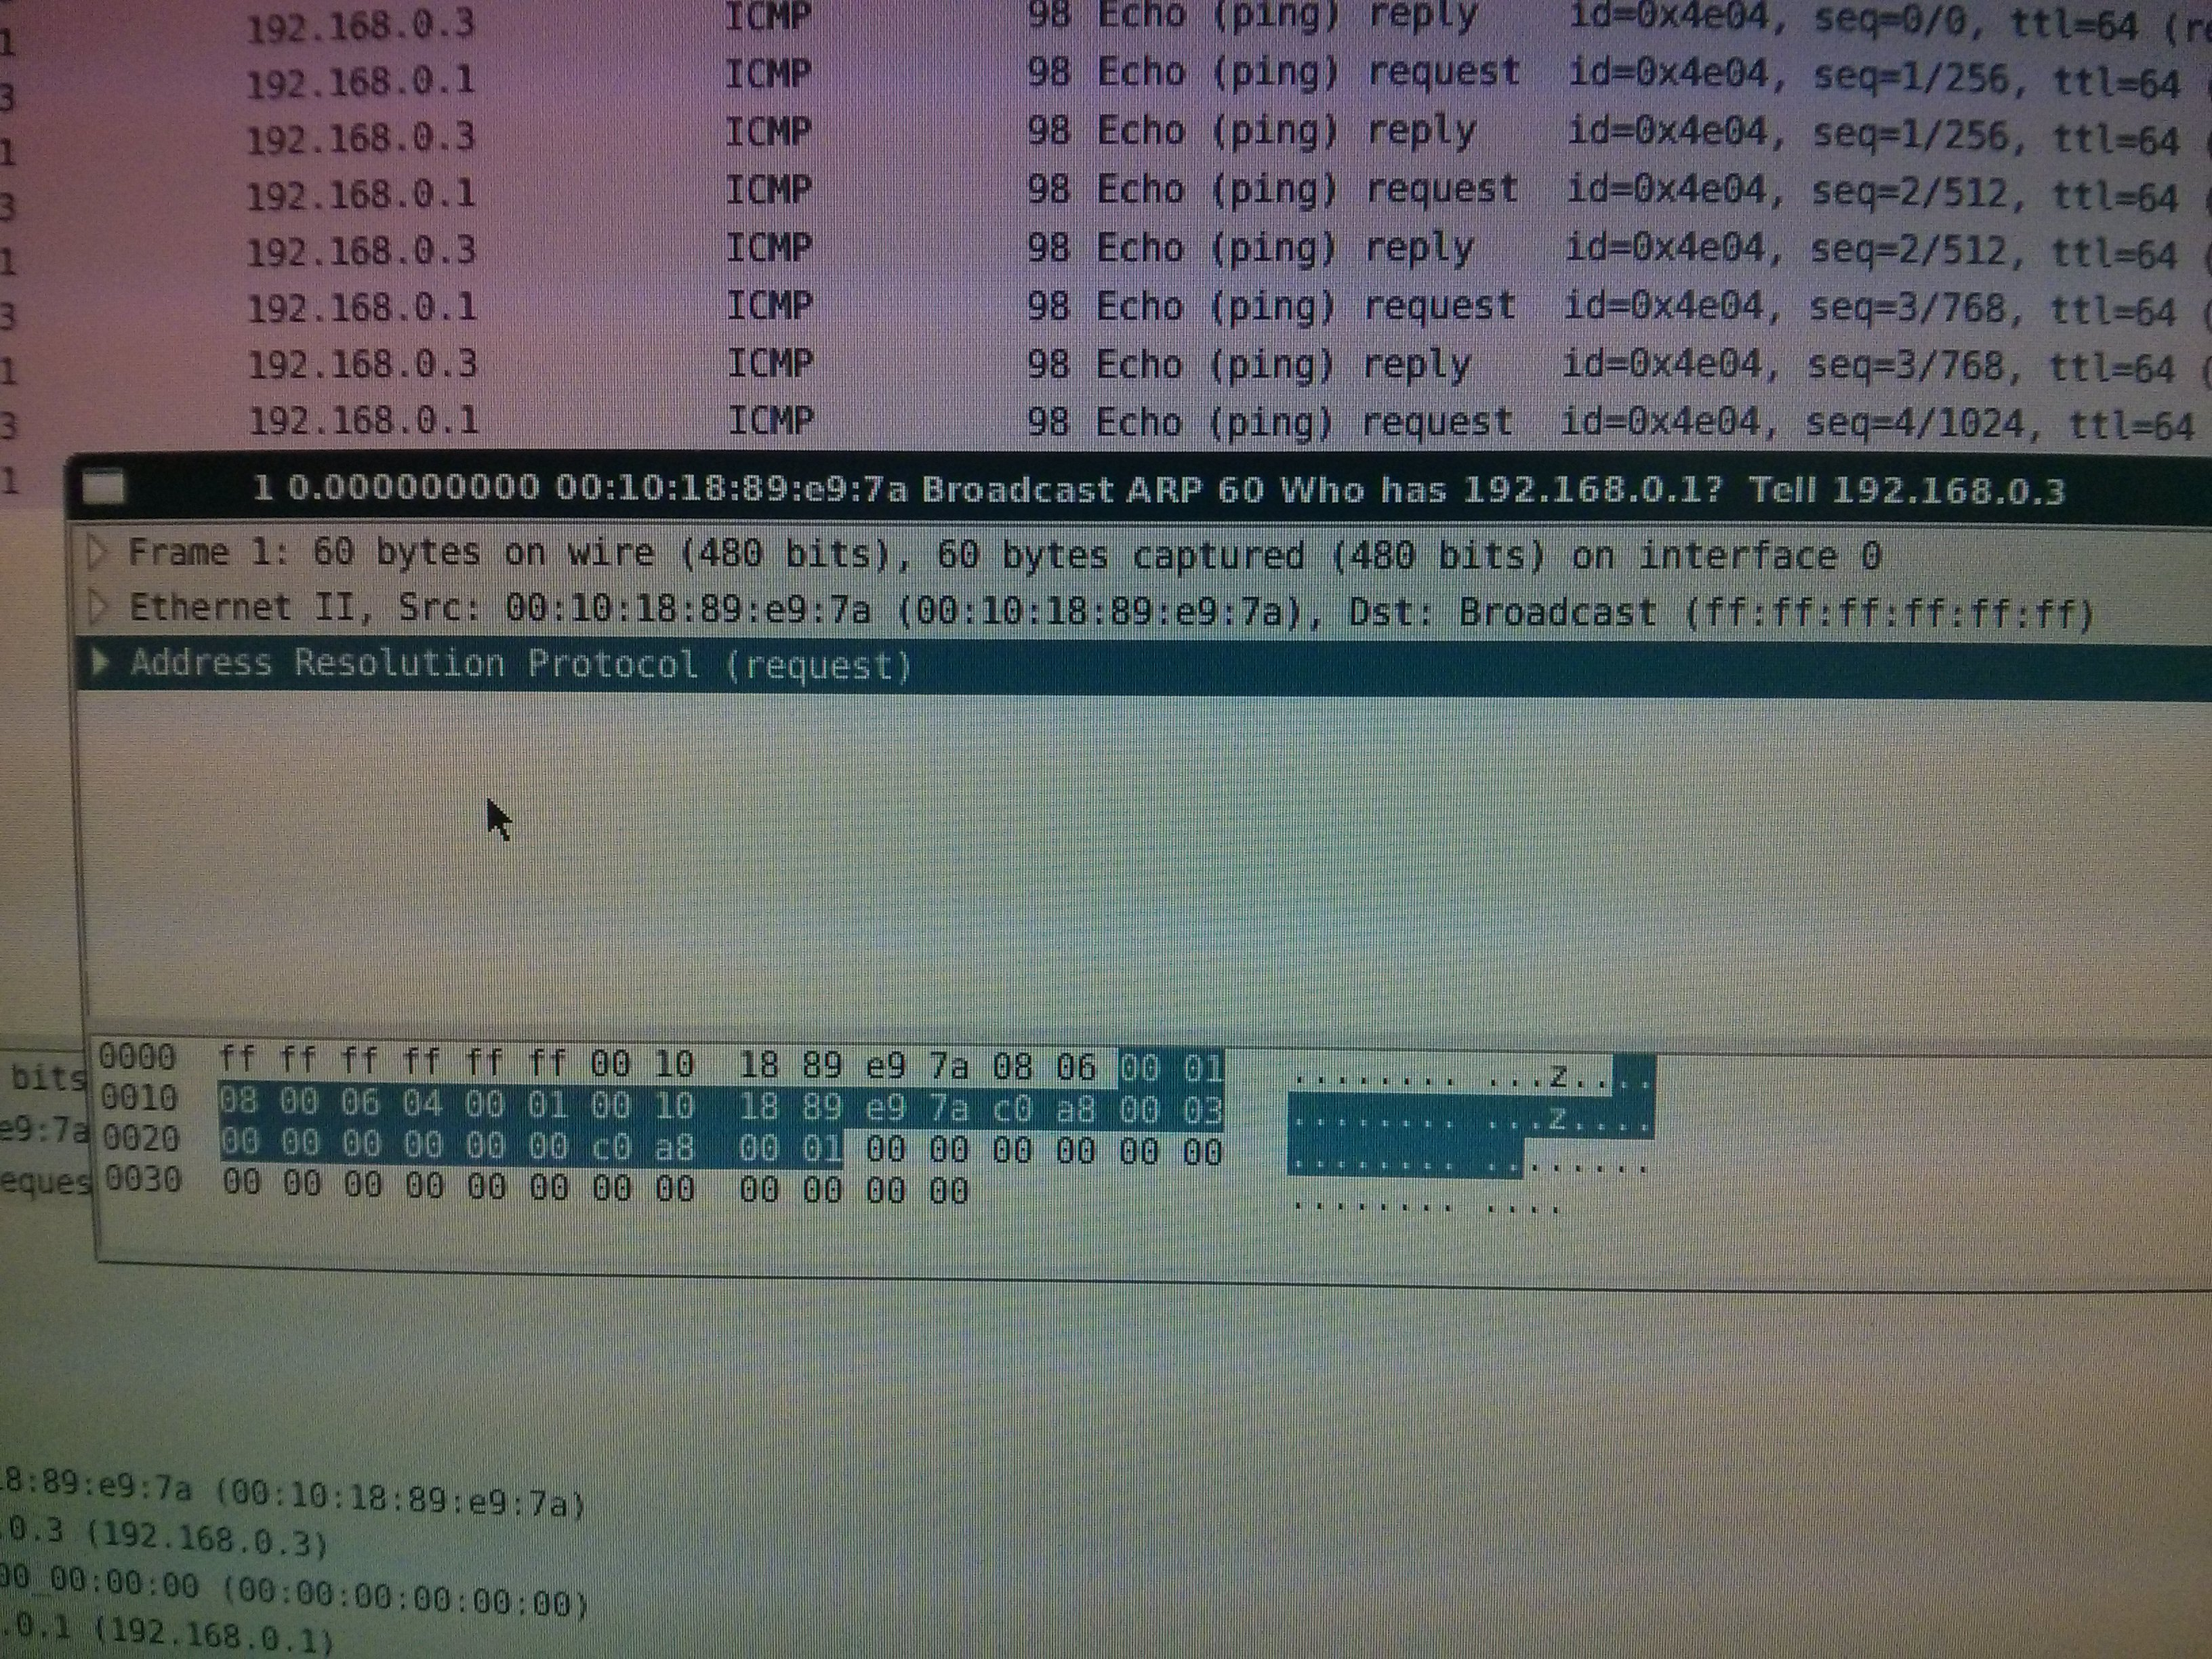
\includegraphics[width=10cm]{screen2.jpg}

	\item 

\begin{tabular}{|p{1.3cm}|p{1.3cm}|p{1.3cm}|p{1.3cm}|p{1.3cm}|p{1.3cm}|p{1.3cm}|p{1.3cm}|p{1.3cm}|}
\hline
Hardware Type (2) &
Protocol Type (2) &
Hardware size (1) &
Protocol size (1) &
Opcode (2) &
Sender MAC address (6) &
Sender IP address (4) &
Target MAC address (6) &
Target IP address (4) \\
\hline
\end{tabular}

	\item Grâce à la longueur du padding, le niveau Ethernet peut déterminer la taille des paquets qu'il reçoit car les données vont écraser le padding (composé uniquement de 00) mais pas forcément le compléter entièrement.
	\item Les octets de bourrage correspondent aux 18 derniers octets de notre trame. (champ padding de l'entête Ethernet)
	\item La couche Ethernet transmet la source du paquet et son destinataire. Ethernet ne connaît pas l'existence d'un bourrage à la réception du paquet car c'est la couche réseau qui se charge du  padding.
\end{itemize}

\subsubsection*{\underline{Algorithme du protocole ARP}}

\begin{enumerate}[label=\arabic*)]
	\item
	\begin{itemize}\renewcommand{\labelitemi}{$\bullet$}
		\item B apparait dans la table de A car A a envoyé une demande pour identifier l'adresse MAC de B sur le broadcast. Et B a envoyé une réponse directement à A avec son adresse MAC. B a pu apprendre l'adresse MAC de A car la requête ARP de A contient son adresse MAC ainsi que son adresse IP.

		\item B ne connait pas l'adresse MAC de A donc cette fois, il envoit un paquet de type ARP au broadcast pour récupérer l'adresse MAC de A.
	\end{itemize}

	\item Dans la table ARP, les adresses MAC des autres stations enregistrées par une station ont un temps d'expiration d'environ 1200 secondes.
	
	\item
	\begin{itemize}\renewcommand{\labelitemi}{$\bullet$}
		\item On constate que A envoit en boucle des paquets de type ARP au broadcast sans avoir de réponse. (On a ensuite le message host is down en boucle)
		\item C'est le timer de Ping qui déclenche les re-émissions. On a constaté que Ping a essayé d'envoyer 10 paquets or on voit bien que dans Wireshark, il y a 10 paquets de type ARP request. A chaque fois que Ping affiche host is down on voit apparaître dans Wireshark un paquet de type ARP request. Le temps de ré-émission est d'environ 1 seconde.

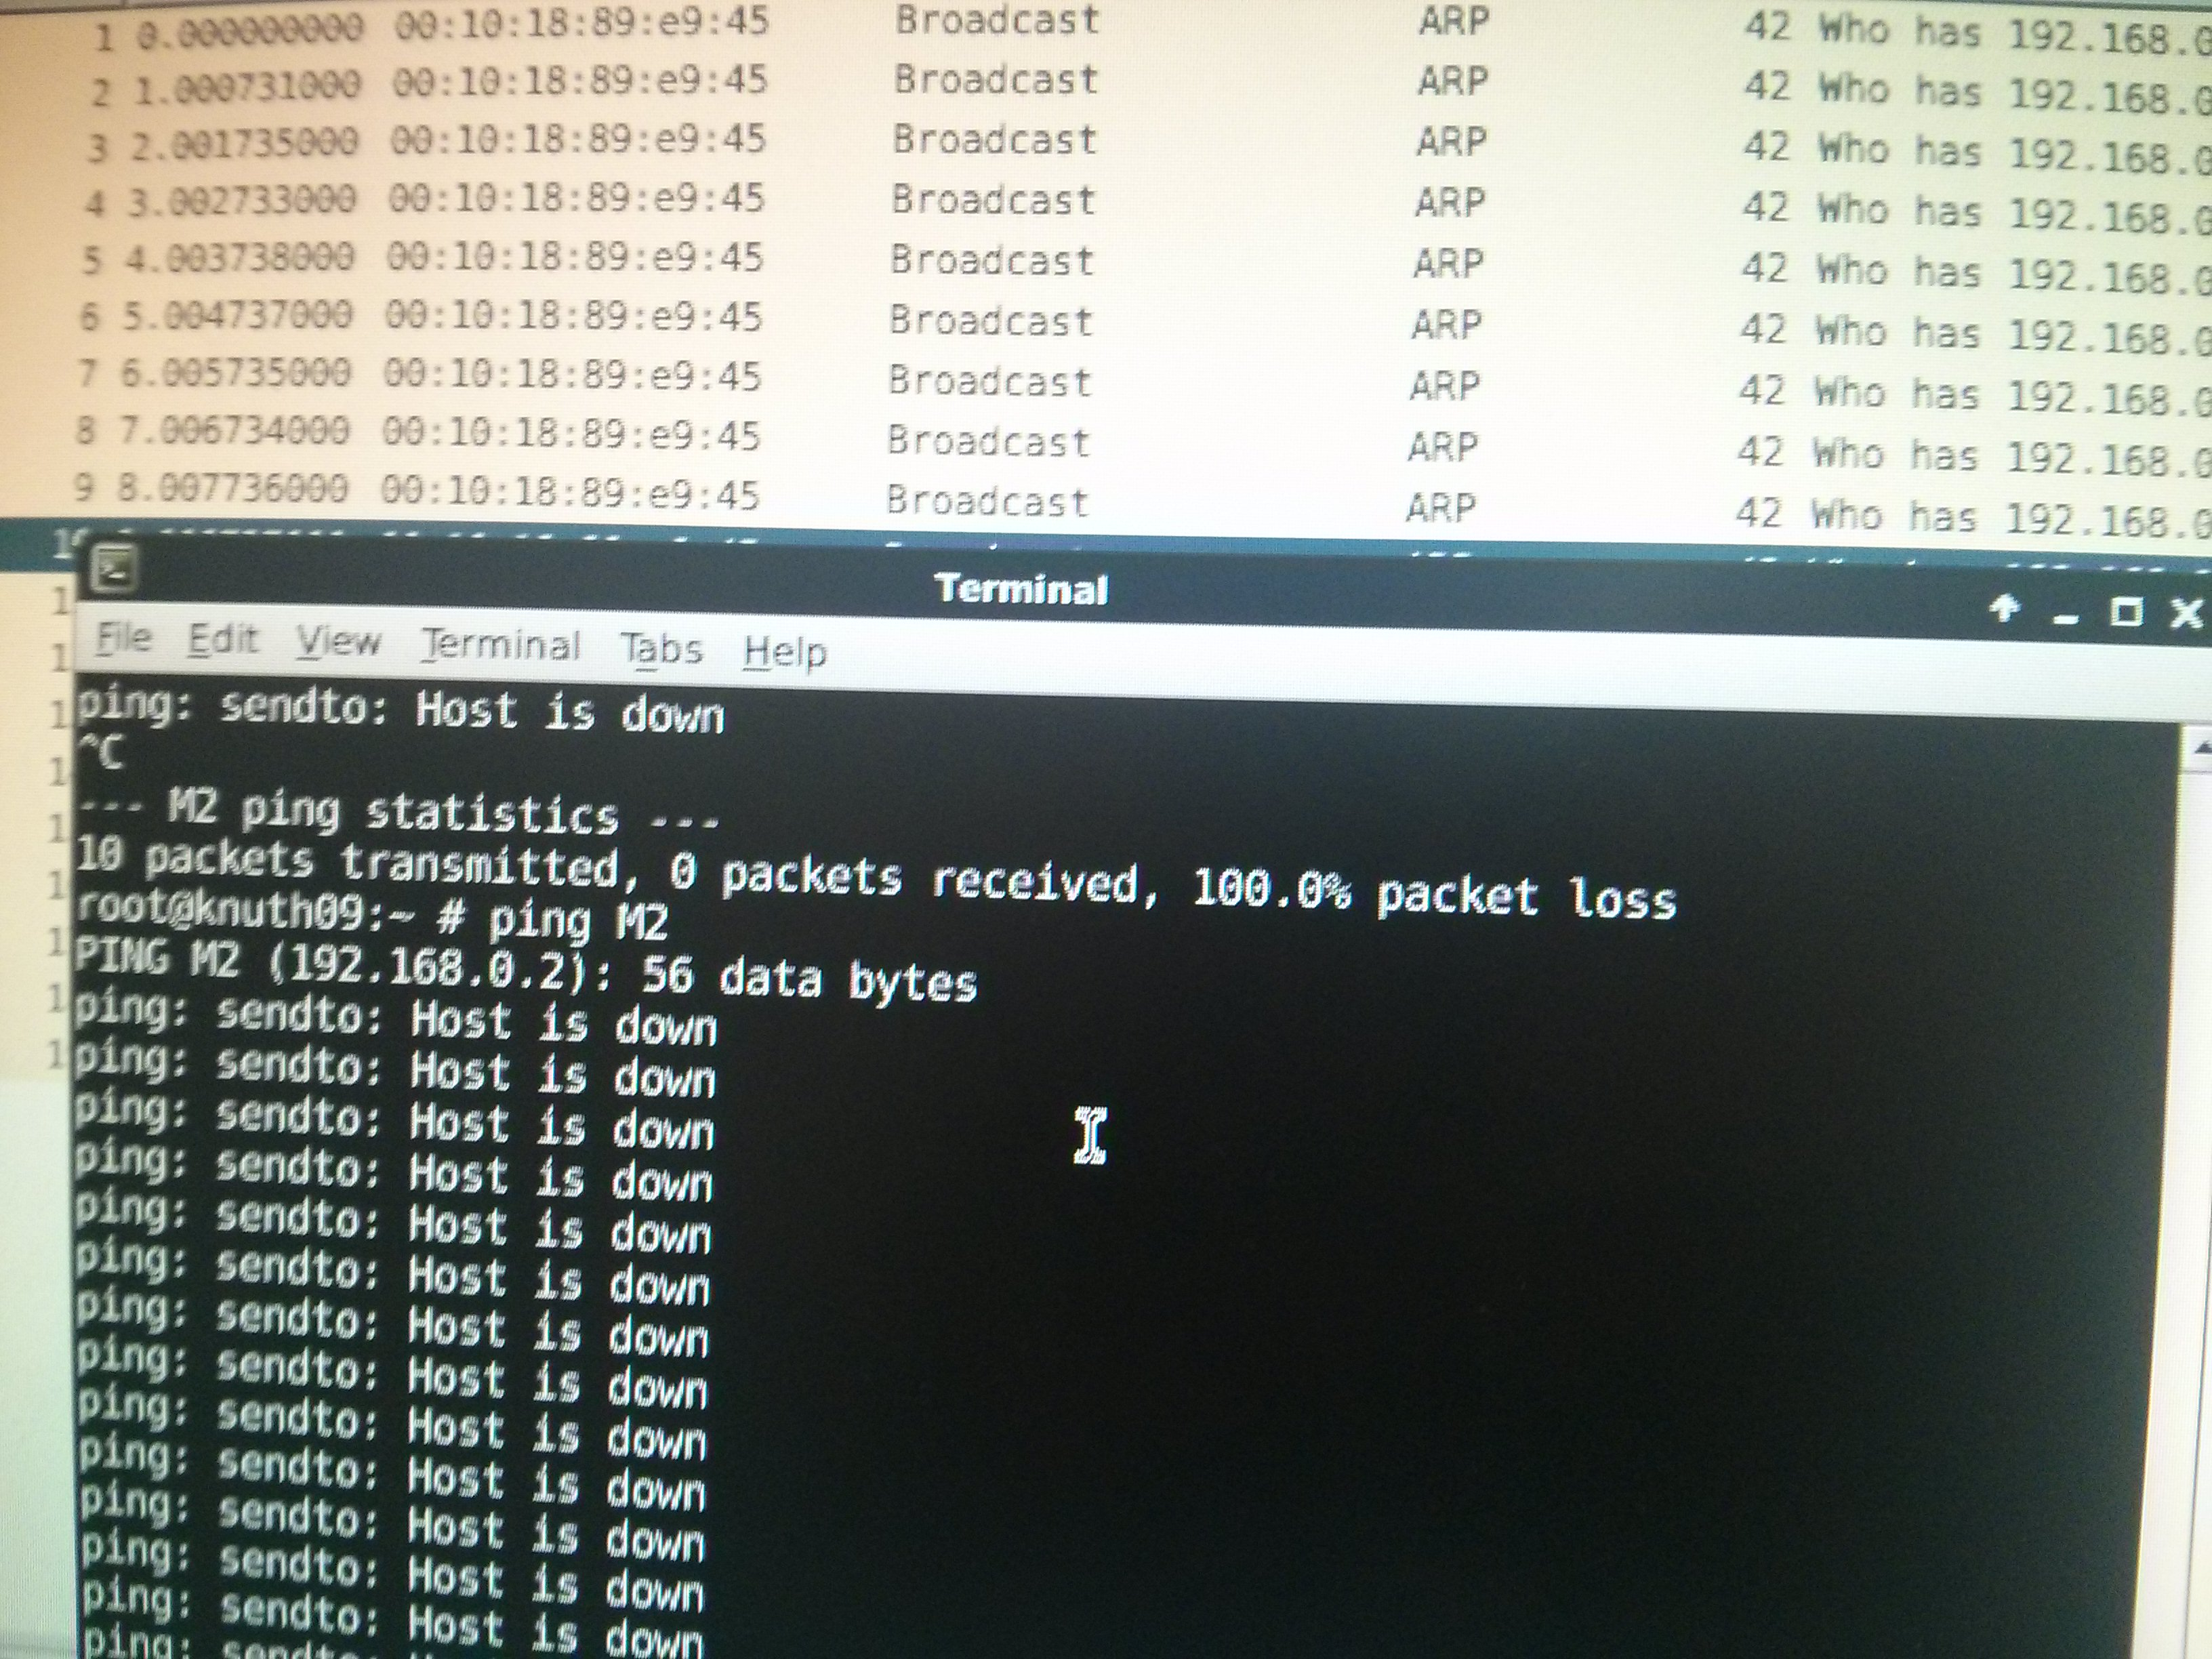
\includegraphics[width=10cm]{screen3.jpg}

	\end{itemize}
	
	\item Le ARP gratuit permet à la machine qui vient d'effectuer un ifconfig de s'envoyer à elle même son adresse MAC sur le réseau et donc lui permet de remplir sa table ARP avec sa propre adresse en vérifiant que cette adresse n'est pas déjà présente (permet d'éviter les conflits d'adresses).

	\item
	\begin{itemize}\renewcommand{\labelitemi}{$\bullet$}
		\item Au moment de la nouvelle entrée dans la table ARP de A, on constate que A a envoyé un paquet de type ARP gratuit à lui même sur le réseau pour ajouter cette nouvelle adresse dans la table.

		\item Au moment du ping de C vers B, on observe 3 paquets de type ARP envoyés sur le réseau. Le premier étant un paquet request envoyé par C au broadcast, puis un paquet reply envoyé par A à C (qui l'informe de l'adresse MAC de B) et enfin un paquet reply envoyé par B à C (qui l'informe aussi de sa propre adresse). 

Dans la table de A, on a les adresses de A et B (B étant en permanent published).

Dans la table de B, on a les adresses de B et C (C qui doit expirer dans X secondes).

Dans la table  de C, on a les mêmes entrées que dans B. A possède l'adresse de B en published, donc quand il observe un ARP request sur le réseau, il y répond et envoit un ARP reply directement à la source de l'ARP request. (et B fait de même)

		\item Au moment de l'ajout dans A de l'adresse IP de B avec l'adresse MAC de A, on constate que A envoit sur le réseau un paquet de type ARP gratuit request mais avec une détection d'un usage dupliqué de l'adresse IP de B. 

Et on voit ensuite un paquet du même type envoyé par B à A. Lors du ping de C vers B, on observe que dans Wireshark il n'y a pas de réponse trouvée pour le ping.
		\item Une déclaration d'adresse en \textit{Publish} d'une autre machine peut être intéressant pour que la machine en question puisse servir de pont entre deux réseaux différents. La machine pourra répondre aux requêtes ARP d'une machine qui ne sera pas sur le même réseau qu'elle.
	\end{itemize}

	\item Au moment où on veut configurer la deuxième machine, on obtient un message système envoyé par le noyau qui nous informe d'un conflit d'adresse IP sur le réseau. 

Au moment d'un ping vers l'adresse IP commune, les deux machines avec l'adresse commune répondent toutes deux au ping une fois mais la dernière a répondre sera le destinataire pour toutes les autres requêtes. (et répondra à chacune d'entre elles tandis que l'autre ne répondra plus).\\
\end{enumerate}


\subsection*{\textbf{Algorithme du protocole ARP}}

\RestyleAlgo{boxed}
\begin{algorithm}[H]
\Deb{
        \Tq{Vrai}{
            attendre(evenement)\;
            \Si{evenement == "Question sur adresse internet" (requête interne de IP vers ARP)}{
		envoiARP(request,IPbroadcast, IPtarget, IPsource, MACsource)\; 

                     	\tcc{Envoi d'une requête ARP sur le broadcast, IPtarget est l'ip du destinataire, Ipsource l'ip de l'expéditeur et MACsource l'adresse MAC de l'expéditeur}\
                }
                \Si{evenement == "Expiration du timer d'effacement associé à une entrée"}{
                        envoiRequeteAdresseInternet()\;
                }
                \Si{evenement == "Réception requête (ARP Request)"}{
                        \Si{IPtarget == IPmachinecourante OU estPublish(IPtarget)}{
			envoiARP(reply, IPtarget, MACtarget, IPsource, MACsource);

			\tcc{IPtarget et MACtarget correspondent aux adresses IP et MAC du destinataire (la machine ayant envoyé l'ARP request)}
			\tcc{IPsource et MACsource correspondent aux adresses IP et MAC de l'expéditeur (adresses présentes dans la table ARP de la machine actuelle)}

			majTableARP(IParget, MACtarget);

			\tcc{la machine actuelle met à jour sa table ARP avec les adresses IP et MAC de l'expéditeur de l'ARP request}
                        }
                    \Sinon{
                      rien\;
                    }
                }
                
                \Si{evenement == "Changement de la configuration internet"}{
                    envoiARP(gratuit)\;
                }
        }
}
\end{algorithm}

\subsection*{2.1.2 Le protocole ICMP}

Notre fichier est de la forme suivante :
\begin{verbatim}
x08 x00			\\ Type Code
x00 x00			\\ CheckSum
x25 x52			\\ Identifier
x25 x52			\\ Sequence Number
x42 x42			\\ Data optionnal
x42 x42			\\ Data optionnal
\end{verbatim}

\begin{itemize}\renewcommand{\labelitemi}{$\bullet$}
	\item On constate qu'on a un premier Identifier (BE) avec pour valeur 9554 (0x2552), un deuxième Identifier (LE) avec pour valeur 21029 (0x5225), un premier Sequence number (BE) avec la même valeur que Identifier (BE) et un deuxième Sequence number (LE) avec la même valeur que Identifier (LE). Ces champs permettent de faire correspondre la requête avec la réponse.
	\item On fait l'addition de nos colonnes et on obtient xD7 x28. Sur un octet cela correspond à 1101 0111 et 0010 1000. On fait le complément à 1 de ces deux nombres, ce qui donne : 0010 1000 et 1101 0111 ce qui nous donne 28 d7 (voir photo ci-dessous). C'est bien le checksum calculé. Ce type de vérification permet de vérifier les rafales d'erreurs inférieures ou égales à la taille du mot (ici 16).
\end{itemize}

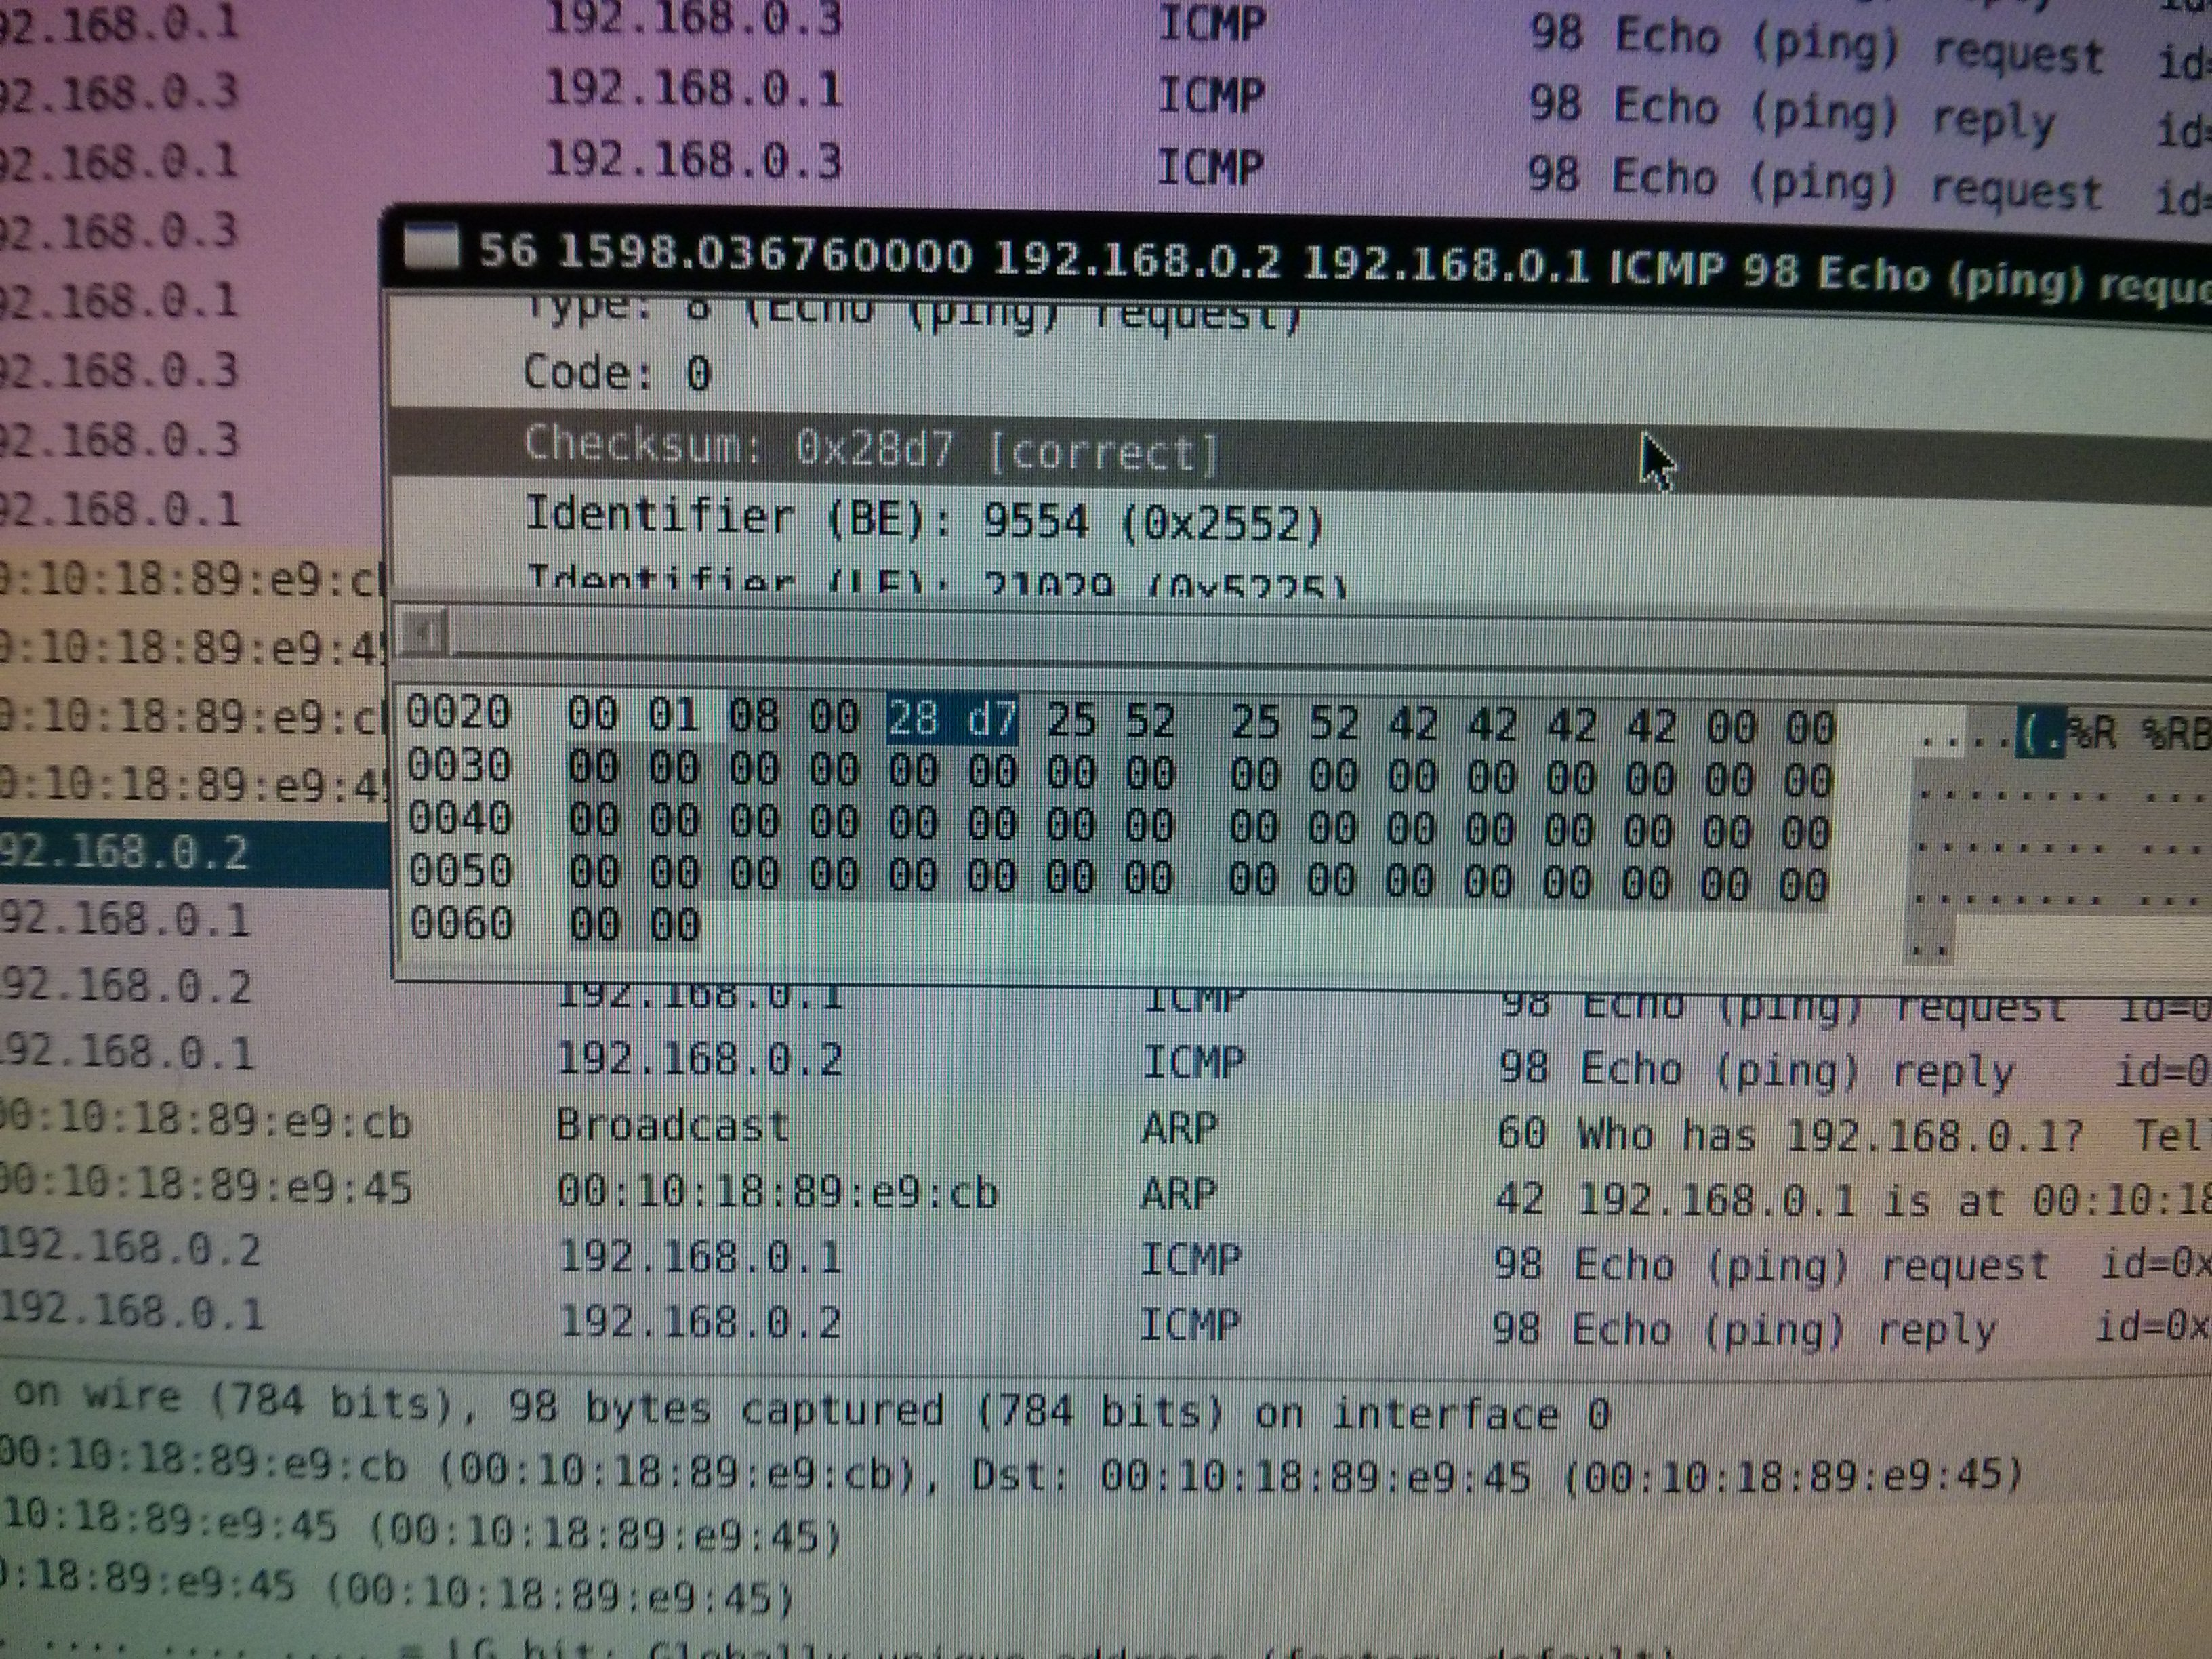
\includegraphics[width=10cm]{screen5.jpg}
\section*{2.2 Etude du protocole DHCP}

DHCP ACK : protocole UDP.
Sur l'interface em0, la machine connectée s'est vu attribuer une adresse IP d'office (ici 152.77.84.11)

\begin{itemize}\renewcommand{\labelitemi}{$\bullet$}
	\item  Client IP address: 0.0.0.0 (0.0.0.0)
	\item  Your client IP address: 152.77.84.11 (152.77.84.11)
	\item  Next server IP address: 152.77.84.125 (152.77.84.125)
	\item  Relay agent IP address: 0.0.0.0 (0.0.0.0)
	\item  Client MAC address: 18 :03 :73 :c7 :b8 :7f (18 :03 :73 :c7 :b8 :7f)
	\item Client hardware address padding: 00000000000000000000
	\item  Server host name not given
	\item  Boot file name: pxeboot-f8
	\item  Magic Cookie: DHCP
	\item  Option: (53) DHCP Message Type (ACK)
	\begin{itemize}
		\item Length :1
		\item DHCP : ACK (5)
	\end{itemize}
	\item  Option: (54) DHCP Server Identifier
	\begin{itemize}
		\item Length : 4
		\item DHCP Server Identifier : 152.77.84.125 (152.77.84.125)
	\end{itemize}
	\item  Option: (51) IP Address Lease Time
	\begin{itemize}
		\item Length: 4
		\item IP Address Lease Time: (600s) 10 minutes
	\end{itemize}
	\item  Option: (1) Subnet Mask
	\begin{itemize}
		\item Length: 4
		\item Subnet Mask: 255.255.255.128 (255.255.255.128)
	\end{itemize}
	\item  Option: (28) Broadcast Address
	\begin{itemize}
		\item Length : 4
		\item Broadcast Address: 152.77.84.127 (152.77.84.127)
	\end{itemize}
	\item  Option: (3) Router
	\begin{itemize}
		\item Length: 4
		\item Router: 152.77.84.1 (152.77.84.1)
	\end{itemize}
	\item  Option: (15) Domain Name
	\begin{itemize}
		\item Length: 17
		\item Domain Name: e.ujf-grenoble.fr
	\end{itemize}
	\item  Option: (6) Domain Name Server
	\begin{itemize}
		\item Length: 8
		\item Domain Name Server: 152.77.24.211 (152.77.24.211)
		\item Domain Name Server: 152.77.24.219 (152.77.24.219)
	\end{itemize}
	\item Option: (12) Host Name
	\begin{itemize}
		\item Length: 25
		\item Host Name: knuth09.e.ujf-grenoble.fr
	\end{itemize}
	\item Option: (255) End
	\begin{itemize}
		\item Option End: 255
	\end{itemize}
	

\end{itemize}

\section*{2.3 Etude de fragmentation des paquets IP}

\begin{itemize}\renewcommand{\labelitemi}{$\bullet$}
	\item Les champs :
	\begin{itemize}
		\item IDENTIFICATION : champ codé sur 16 bits, constitue l'identification utilisée pour reconstituer les fragments. (Les fragments ont tous le même numéro d'identification)
		\item TOTAL LENGTH : champ codé sur 16 bits, correspond à la longueur du paquet (entête IP + données)
		\item FRAGMENT OFFSET : champ codé sur 13 bits, correspond à la position du fragment (par rapport à la première trame).
		\item Flag MF : More Fragments => si le troisième bit est à 1, indique que le fragment n'est pas le dernier
	\end{itemize}
	\item L'entête UDP apparaît une seule fois car il n'y a qu'un seul paquet de type UDP. Les fragments, eux, sont des données IP.
	\item Les fragments sont envoyés dans le même ordre que celui du paquet d'origine.
	\item L'entête UDP se trouve dans le dernier fragment.
\end{itemize}



\end{document}